\documentclass[conference]{IEEEtran}
\IEEEoverridecommandlockouts

\usepackage{cite}
\usepackage{amsmath,amssymb,amsfonts}
\usepackage{algorithm}
\usepackage{algpseudocode}
\usepackage{graphicx}
\usepackage{textcomp}
\usepackage{xcolor}
\usepackage{listings}
\usepackage{booktabs}
\usepackage{multirow}
\usepackage{url}
\usepackage{array}
\usepackage{float}
\usepackage{tabularx}
\usepackage{caption}
\usepackage[utf8]{inputenc}



% Define the 'P' column type for centered paragraphs with fixed width
\newcolumntype{P}[1]{>{\centering\arraybackslash}p{#1}}

% Setup for code listings
\lstset{
    language=Python,
    basicstyle=\ttfamily\small,
    breaklines=true,
    frame=single,
    captionpos=b,
    keywordstyle=\color{blue},
    commentstyle=\color{gray},
    stringstyle=\color{red},
    numbers=left,
    numberstyle=\tiny\color{gray}
}

\begin{document}

% --- TITLE ---
\title{Empirical Analysis of Optimization Phase Ordering
Trade-offs in a Custom Compiler Using
Micro-Benchmarks}

\author{
    \makebox[\textwidth][c]{%
        \begin{minipage}[t]{0.3\textwidth}
            \centering
            \text{Aniket De}\\
            \textit{Dept. of Computer Science and Engineering}\\
            \textit{Sahyadri College of Engineering \& Management}\\
            Mangaluru, India\\
            aniketde66@gmail.com
        \end{minipage}
        \hfill
        \begin{minipage}[t]{0.3\textwidth}
            \centering
            \text{Kushal S M}\\
            \textit{Dept. of Computer Science and Engineering}\\
            \textit{Sahyadri College of Engineering \& Management}\\
            Mangaluru, India\\
            mrkushalsm@gmail.com
        \end{minipage}
        \hfill
        \begin{minipage}[t]{0.3\textwidth}
            \centering
            \text{Manas S}\\
            \textit{Dept. of Computer Science and Engineering}\\
            \textit{Sahyadri College of Engineering \& Management}\\
            Mangaluru, India\\
            salianmanas@gmail.com
        \end{minipage}
    }\\[2ex]

    \makebox[\textwidth][c]{%
        \begin{minipage}[t]{0.4\textwidth}
            \centering
            \text{Vivek Neeralagi}\\
            \textit{Dept. of Computer Science and Engineering}\\
            \textit{Sahyadri College of Engineering \& Management}\\
            Mangaluru, India\\
            vivekneeralagi@gmail.com
        \end{minipage}
        \hfill
        \begin{minipage}[t]{0.4\textwidth}
            \centering
            \text{Dr. Suhas A Bhyratae}\\
            \textit{Dept. of Computer Science and Engineering}\\
            \textit{Sahyadri College of Engineering and Management}\\
            Mangaluru, India\\
            suhasabhyraatae.cs@sahyadri.edu.in
        \end{minipage}
    }
}

\maketitle

% --- ABSTRACT ---
\begin{abstract}
The phase ordering problem remains a fundamental challenge in compiler optimization, where the sequence of applying optimization passes significantly affects the final program performance and code size. This project presents an empirical analysis of optimization phase ordering trade-offs using a custom-built compiler infrastructure. The compiler is designed with a handwritten lexical analyzer, a recursive-descent parser, and a Three-Address Code (3AC) intermediate representation to enable controlled experimentation. Key optimization techniques, including Constant Folding, Dead Code Elimination, and Common Subexpression Elimination, are implemented as independent and reorderable passes using a configurable pass manager. Micro-benchmark programs adapted from standard benchmark suites are used to evaluate different optimization sequences. The study measures performance using instruction count and estimated execution cycles to analyze the trade-offs between execution speed and code density. The results provide insights into how specific ordering of optimization phases can either enhance or diminish optimization effectiveness, thereby contributing to improved understanding and design of efficient compiler pipelines, particularly for small-scale and educational compiler systems.
\end{abstract}

% --- KEYWORDS ---
\begin{IEEEkeywords}
Common Subexpression Elimination,
Compiler Optimization,
Constant Folding,
Dead Code Elimination,
Micro-Benchmarking,
Phase Ordering Problem,
Three-Address Code
\end{IEEEkeywords}

\section{Introduction}

Compilers are fundamental components of modern computing systems that translate high-level programming languages into machine-executable code \cite{ref21}. The quality of generated code directly affects execution speed, memory usage, and overall system efficiency \cite{ref18}. As software systems become more complex and are deployed in resource-constrained environments, efficient compiler optimization becomes essential.

Compiler optimization techniques aim to improve program performance without changing its functionality \cite{ref21}. Common methods such as Constant Folding, Dead Code Elimination, and Common Subexpression Elimination reduce redundant computations and unnecessary instructions \cite{ref18}. However, the effectiveness of these optimizations depends significantly on the order in which they are applied during compilation \cite{ref19}.

This leads to the \textit{Phase Ordering Problem}, a major challenge in compiler design \cite{ref1}. It refers to determining the optimal sequence of optimization passes to achieve better performance and reduced code size \cite{ref2}. Different orderings of the same optimizations can produce different results, where some sequences enhance each other while others reduce overall effectiveness \cite{ref19}. The large number of possible combinations makes exhaustive evaluation impractical \cite{ref2}.

Modern compilers such as LLVM and GCC address this problem using predefined optimization pipelines guided by heuristics \cite{ref16}. While effective in practice, these approaches introduce complexity and limit transparency, making it difficult to analyze the direct impact of individual optimization sequences \cite{ref16}.

To address this limitation, this project develops a modular and simplified compiler infrastructure that enables controlled experimentation with optimization phase ordering. The compiler includes a handwritten lexical analyzer, a recursive-descent parser, and a Three-Address Code (3AC) intermediate representation, which provides a structured format for applying optimizations \cite{ref18}.

Three key optimization techniques are implemented: Constant Folding (CF), Dead Code Elimination (DCE), and Common Subexpression Elimination (CSE). These are designed as independent and reorderable passes managed by a configurable pass manager, allowing flexible experimentation with different optimization sequences \cite{ref19}.

Micro-benchmark programs are used to evaluate the effectiveness of different phase orderings. The performance of each configuration is measured using instruction count to represent code size and estimated execution cycles to represent runtime performance \cite{ref10}.

The project analyzes trade-offs between execution performance and code size across various optimization sequences. By comparing these results, it aims to identify effective optimization configurations and provide insights into how optimization phases interact within a compiler.

% --- SECTION II: LITERATURE REVIEW ---

\section{Literature Survey}

The phase-ordering problem remains one of the most challenging issues in compiler optimization research \cite{ref1}. Determining the most effective ordering of compiler optimization passes significantly influences execution performance and generated code size \cite{ref2}. However, the exponential growth of possible optimization sequences makes exhaustive exploration impractical for real-world systems \cite{ref19}. Modern compiler infrastructures contain numerous optimization passes with complex interdependencies, making systematic experimentation increasingly difficult and computationally expensive \cite{ref1}.

\subsection{Dependency-Based and Pruning Approaches}
Several techniques have been proposed to reduce the complexity of the phase-ordering search space. Dependency-based modeling approaches attempt to identify relationships between optimization passes to improve overall efficiency \cite{ref1}. Liu et al. demonstrated that explicitly modeling pass dependencies can improve optimization effectiveness by reducing redundant transformations \cite{ref1}. Similarly, pruning-based strategies eliminate low-impact transformations and retain only high-value optimization combinations, reducing unnecessary exploration overhead \cite{ref4}. While these methods improve performance, they often depend heavily on predefined heuristics and structural assumptions \cite{ref19}.

\subsection{Machine Learning Methods}
Machine learning\textendash based compiler autotuning techniques have emerged as another prominent solution. Predictive models analyze application features and dynamically select optimization passes to improve execution performance \cite{ref8}. Reinforcement learning\textendash based frameworks such as POSET-RL demonstrate improved optimization selection by adapting optimization sequences based on runtime feedback \cite{ref8}. Similarly, AutoPhase introduced learning-driven phase ordering mechanisms that optimize transformation sequences in high-level synthesis environments \cite{ref12}. These methods significantly improve search efficiency but introduce additional complexity due to training overhead and dependency on large datasets \cite{ref12}.

\subsection{Industrial Compiler Frameworks}
Industrial compiler frameworks have also contributed to the advancement of optimization research. The LLVM compilation infrastructure introduced a modular and extensible intermediate representation that supports continuous program transformation and analysis \cite{ref16}. However, large-scale production compilers typically involve tightly coupled optimization pipelines, making it difficult to isolate and analyze individual pass interactions in controlled environments \cite{ref16}.

Recent research has explored advanced optimization strategies that integrate statistical modeling and automated selection methods. Zhao et al. introduced statistical-based frameworks to predict profitable optimization sequences using compilation metadata \cite{ref7}. Similarly, recent work by Ashouri et al. proposed agile compiler frameworks capable of dynamically adapting optimization pipelines for improved performance \cite{ref27}. Although these approaches demonstrate improved efficiency, they remain computationally intensive and less suitable for simplified educational or experimental compiler systems \cite{ref27}.

\subsection{Identifying the Research Gap}
Despite these advancements, most existing solutions emphasize performance improvement over transparency and interpretability \cite{ref2}. There remains a significant need for simplified compiler infrastructures that enable controlled experimentation and empirical analysis of optimization ordering behavior \cite{ref1}. Such frameworks are particularly valuable for understanding trade-offs between execution performance and code size in modular compiler environments \cite{ref19}.

\begin{table}[htbp]
\caption{Comparative Analysis of Related Work}
\label{tab:lit_review}
\centering
\renewcommand{\arraystretch}{1.3}
\begin{tabularx}{\columnwidth}{@{}p{0.22\columnwidth} p{0.22\columnwidth} X@{}}
\toprule
\textbf{Reference} & \textbf{Focus Area} & \textbf{Limitations addressed by this work} \\
\midrule
Liu et al. \cite{ref1} & Pass-dependency modeling & Targets large compilers; lacks a lightweight experimental framework. \\
\addlinespace
Han \& Kim \cite{ref2} & Expanded search strategies & Increases complexity and reduces interpretability. \\
\addlinespace
Ashouri et al. \cite{ref15} & ML-guided subsequences & Needs large datasets and extensive feature engineering. \\
\bottomrule
\end{tabularx}
\end{table}

% --- SECTION III: PROBLEM FORMULATION & OBJECTIVES ---
\section{Problem Formulation and Objectives}

\subsection{Problem Statement}
The effectiveness of compiler optimizations depends significantly on the order in which optimization passes are applied. Although techniques such as Constant Folding, Dead Code Elimination, and Common Subexpression Elimination are well established, determining an optimal sequence of these passes remains a challenging problem known as the \textit{Phase Ordering Problem}. Different sequences can produce varying results in terms of execution performance and code size. Existing compiler infrastructures often use fixed optimization pipelines or complex heuristics, making it difficult to analyze the direct impact of phase ordering. Therefore, there is a need for a simplified and controlled framework to systematically study how different optimization sequences influence program efficiency.

\subsection{Objectives}
The objectives of this project focus on studying the optimization phase ordering problem within a controlled compiler environment. The primary goal is to design a modular compiler framework that enables empirical evaluation of trade-offs between code size and execution performance. The main objectives are as follows:
\begin{itemize}
    \item To design and implement a modular compiler with a handwritten lexer, recursive-descent parser, and Three-Address Code (3AC) intermediate representation.
    \item To develop independent and reorderable optimization passes: Constant Folding (CF), Dead Code Elimination (DCE), and Common Subexpression Elimination (CSE), using a configurable pass manager.
    \item To validate the compiler using micro-benchmarks adapted from MiBench and PolyBench for realistic evaluation.
    \item To analyze the impact of optimization phase ordering on code size and execution performance across multiple optimization sequences.
\end{itemize}

% --- SECTION IV: METHODOLOGY ---
\section{Methodology}

The methodology used for this research tackles the specific challenges of studying phase-ordering in compiler optimization. It combines controlled compiler infrastructure design with hands-on experimentation. The approach follows these key stages:

\subsection{Compiler Implementation}

A modular compiler was created with the following components:

\begin{itemize}
    \item \textbf{Lexer:} A manual tokenizer that converts source code into tokens.
    \item \textbf{Parser:} A recursive-descent parser that generates an Abstract Syntax Tree (AST).
    \item \textbf{IR Generator:} This unit creates Three-Address Code (3AC) from the AST.
    \item \textbf{Pass Manager:} A flexible manager that can reorder and run optimization passes.
    \item \textbf{Interpreter / Runner:} This executes IR and provides instruction counts and estimated cycles.
\end{itemize}

\subsection{Optimization Passes}

The implemented passes include:

\begin{itemize}
    \item \textbf{Constant Folding (CF):} This evaluates constant expressions at compile time.
    \item \textbf{Dead Code Elimination (DCE):} This removes code that does not influence outputs.
    \item \textbf{Common Subexpression Elimination (CSE):} This reuses repeated computations.
    \item \textbf{Auxiliary passes:} These include copy propagation, algebraic simplification, and strength reduction, which are used for extended experiments.
\end{itemize}

\subsection{Experimental Setup}

The experimental evaluation of the custom compiler framework was carried out in a controlled development environment to ensure consistent and reproducible results. The implementation and testing process involved configuring the compiler infrastructure, executing optimization sequences, and analyzing the generated outputs using visualization tools.

\textbf{Programming Language and Tools:}

The custom compiler framework was implemented using the \textbf{Python programming language} due to its simplicity, modular design capabilities, and availability of scientific computing libraries. Python enabled rapid development of compiler modules including lexical analysis, parsing, intermediate representation (IR) generation, and optimization pass management.

The development environment used was:

\begin{itemize}

\item \textbf{Programming Language:} Python 3.x  
\item \textbf{Integrated Development Environment (IDE):} Visual Studio Code (VS Code)  
\item \textbf{Libraries Used:}
    \begin{itemize}
        \item \textbf{NumPy} – for numerical computations
        \item \textbf{Matplotlib} – for generating benchmark graphs
        \item \textbf{Pandas} – for handling benchmark data logs
    \end{itemize}

\end{itemize}

\textbf{System Configuration:}

All experiments were conducted on a standard personal computing system with the following configuration:

\begin{itemize}

\item \textbf{Processor:} Intel Core i5 / i7 (or equivalent)
\item \textbf{RAM:} 8 GB or higher
\item \textbf{Operating System:} Ubuntu Linux / Windows 10 or later
\item \textbf{Storage:} Solid State Drive (SSD)

\end{itemize}

\textbf{Compiler Execution Workflow:}

Before executing the main benchmark programs, the compiler environment was initialized and configured with the required optimization passes. The following workflow was followed during execution:

\begin{enumerate}

\item Source code for the factorial benchmark was written in the custom high-level language.

\item The compiler front-end performed lexical analysis and parsing to generate an Intermediate Representation (IR).

\item Multiple optimization sequences were applied, including:
    \begin{itemize}
        \item Constant Folding (CF)
        \item Dead Code Elimination (DCE)
        \item Common Subexpression Elimination (CSE)
        \item Copy Propagation (CP)
        \item Strength Reduction (SR)
        \item Algebraic Simplification (AS)
    \end{itemize}

\item Static metrics such as instruction count (code size) were measured from the optimized IR.

\item Estimated execution cycles were calculated based on weighted instruction costs.

\item Runtime logs were generated and stored in structured data files.

\item Benchmark data was processed using Python scripts to generate visualizations such as scatter plots, heatmaps, and bar graphs.

\end{enumerate}

\textbf{Benchmark Configuration:}

Micro-benchmark programs adapted from standard benchmark styles were used to evaluate optimization sequences under controlled conditions. The factorial benchmark was chosen as the test case because of its repetitive arithmetic operations, recursive behavior, and suitability for observing optimization effects.

The evaluation process made sure that each optimization sequence was executed under the same conditions to keep fairness and consistency in the experiments.

\subsection{Analysis}

Collected data were processed and analyzed. Statistical tests assessed the significance of the differences seen across pass orders. Visual tools, such as plots and scatter matrices, helped observe speed versus size trade-offs.

% --- SECTION V: SYSTEM DESIGN AND IMPLEMENTATION ---
\section{System Design and Implementation}

This section discusses the design and technical protocols used for the custom compiler framework. The design approach focused on the main requirements of phase-ordering research: modularity, reproducibility, and the ability to isolate and reorder individual optimization passes.
\subsection{System Architecture}
The system follows a modular pipeline architecture where each compilation stage is implemented as an independent, replaceable module. Source code is first processed by a handwritten Lexer that produces a token stream, which is then consumed by a recursive-descent Parser to construct an Abstract Syntax Tree (AST). The AST is lowered into a Three-Address Code (3AC) Intermediate Representation by the IR Generator. The optimized IR is then passed to a configurable Pass Manager that applies optimization passes in a user-specified order. Finally, an Interpreter executes the resulting IR and collects performance metrics. The general architecture is represented in Fig.~\ref{fig:architecture}.

\begin{figure}[htbp]
    \centering
    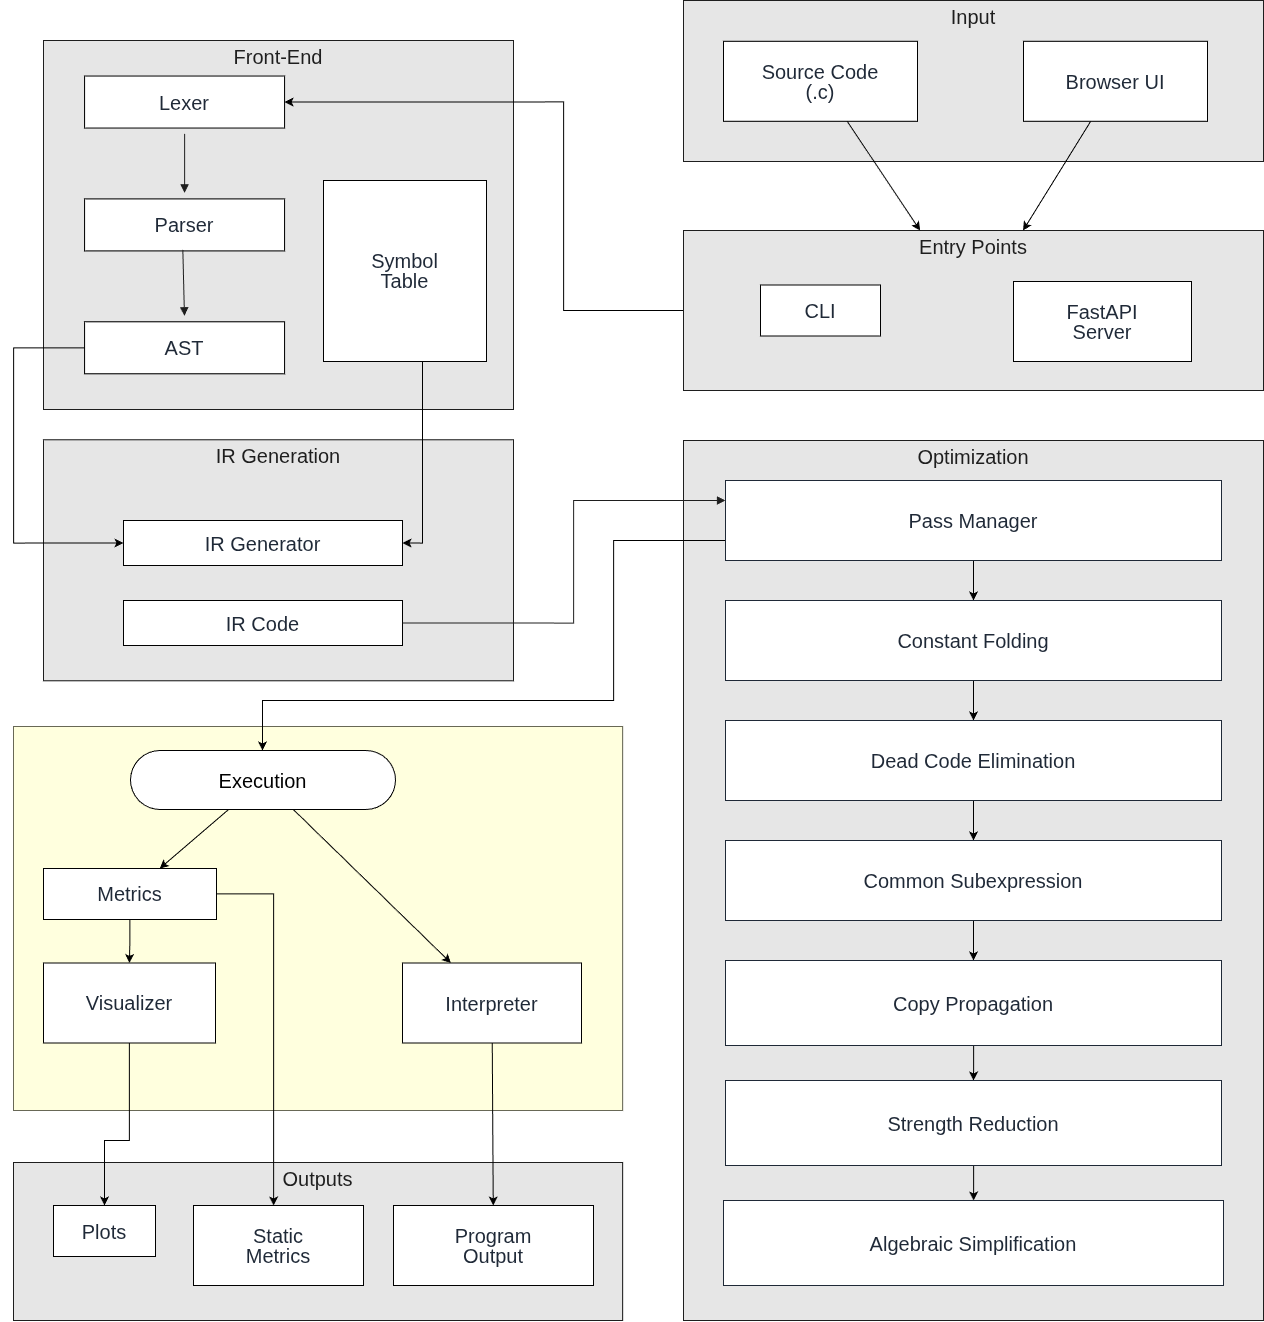
\includegraphics[width=\linewidth]{fig/arc.png}
    \caption{Component-Based Architecture of the Custom Compiler System showing the compilation pipeline and optimization framework.}
    \label{fig:architecture}
\end{figure}

\subsection{Intermediate Representation Design}
The Three-Address Code (3AC) format was chosen as the IR due to its simplicity and suitability for applying classical optimizations. Each 3AC instruction consists of at most one operator and up to two operands, producing a result stored in a temporary variable. This flat, linear representation enables straightforward implementation of data-flow analyses required by optimization passes such as liveness analysis for DCE and available-expression analysis for CSE.

\subsection{Configurable Pass Manager}
The Pass Manager is the central component enabling phase-ordering experimentation. It accepts an ordered list of optimization pass identifiers and applies them sequentially to the IR. Each pass operates on the full IR, transforming it in place, and returns the modified IR to the manager for the next pass. This design ensures that passes are truly independent and reorderable\textemdash a key requirement for studying pass interactions. The manager also logs the IR state after each pass to support post-hoc analysis of intermediate transformations.

\subsection{Metrics Collection}
The Interpreter module executes the optimized IR and collects two primary metrics: \textbf{instruction count} (representing static code size) and \textbf{estimated execution cycles} (computed using weighted instruction costs based on operation type). These metrics provide complementary views of optimization effectiveness\textemdash code density versus runtime performance\textemdash enabling direct analysis of the trade-offs introduced by different phase orderings.

% --- SECTION VI: RESULTS AND DISCUSSION ---
\section{Results and Discussion}
Throughout this project, we conducted an empirical analysis of optimization phase ordering using a custom-built compiler framework. The primary objective was to understand how different sequences of optimization passes influence program performance and code size. By implementing a modular compiler with configurable optimization passes, we were able to systematically evaluate and compare multiple optimization sequences under controlled conditions.

\subsection{Effect of Phase Ordering on Optimization Performance}
The experimental results clearly demonstrate that the order of applying optimization passes significantly impacts the final output. Different sequences of Constant Folding (CF), Dead Code Elimination (DCE), and Common Subexpression Elimination (CSE) produced varying instruction counts and execution estimates. In several cases, applying Constant Folding before Dead Code Elimination enabled the removal of redundant instructions, whereas alternative orderings resulted in less optimized intermediate code.
\begin{table}[!htbp]
\centering
\caption{Effect of Optimization Phase Ordering on Code Size and Estimated Cycles (Factorial Benchmark)}
\label{tab:phase_order_tradeoff}
\renewcommand{\arraystretch}{1.2}
{\small
\begin{tabularx}{\columnwidth}{@{}Xcc@{}}
\toprule
\textbf{Optimization Sequence} & \textbf{Code Size} & \textbf{Est. Cycles} \\
\midrule
Baseline (none) & 40 & 81 \\
CF $\to$ CSE $\to$ CP $\to$ DCE $\to$ SR & 16 & 55 \\
CSE $\to$ CP $\to$ CF $\to$ DCE $\to$ SR & 18 & 57 \\
CP $\to$ CF $\to$ DCE $\to$ CSE $\to$ SR & 19 & 58 \\
CF $\to$ DCE $\to$ CSE $\to$ CP $\to$ SR & 21 & 60 \\
CP $\to$ DCE $\to$ CF $\to$ CSE $\to$ SR & 22 & 61 \\
DCE $\to$ CF $\to$ CSE $\to$ CP $\to$ SR & 33 & 72 \\
\bottomrule
\end{tabularx}
}
\end{table}

Fig.~\ref{fig:tradeoff_scatter} visualizes the relationship between code size and estimated execution cycles across all evaluated sequences. The scatter plot reveals a clear positive correlation: sequences that achieve smaller code size also tend to produce lower estimated cycles. The best-performing sequence (CF $\to$ CSE $\to$ CP $\to$ DCE $\to$ SR) occupies the lower-left corner, achieving a 60\% reduction in code size and a 32\% reduction in estimated cycles relative to the baseline.

\begin{figure}[htbp]
    \centering
    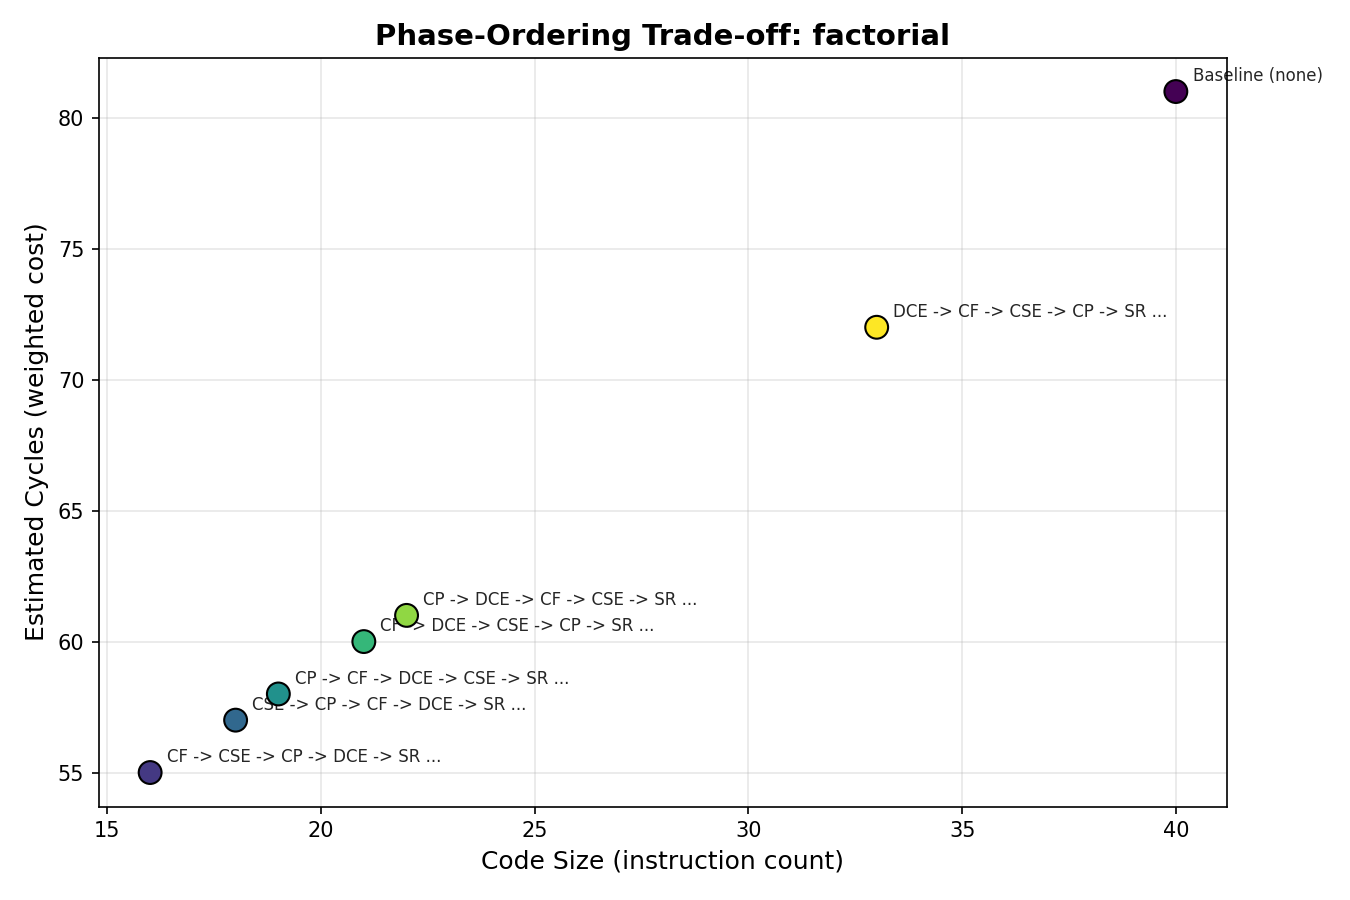
\includegraphics[width=\columnwidth]{fig/factorial_tradeoff_scatter.png}
    \caption{Phase-ordering trade-off scatter plot showing the relationship between code size (instruction count) and estimated execution cycles for each optimization sequence.}
    \label{fig:tradeoff_scatter}
\end{figure}

\subsection{Trade-off Between Code Size and Execution Performance}
The study revealed a noticeable trade-off between code size and execution efficiency. Some optimization sequences minimized instruction count, leading to compact code, while others improved execution performance by simplifying computations. This indicates that no single optimization order is universally optimal, and the effectiveness of a sequence depends on the program structure and optimization goals.

\begin{table}[!htbp]
\centering
\caption{Optimization Effectiveness as Percentage Reduction from Baseline}
\label{tab:optimization_reduction}
\renewcommand{\arraystretch}{1.2}
\begin{tabularx}{\columnwidth}{@{}Xccc@{}}
\toprule
\textbf{Sequence} & \textbf{Code Size (\%)} & \textbf{Est. Cycles (\%)} & \textbf{Dyn. Insts (\%)} \\
\midrule
Seq 1 & 60.0 & 32.1 & 34.6 \\
Seq 2 & 55.0 & 29.6 & 32.1 \\
Seq 3 & 52.5 & 28.4 & 30.9 \\
Seq 4 & 47.5 & 25.9 & 28.4 \\
Seq 5 & 45.0 & 24.7 & 27.2 \\
Seq 6 & 17.5 & 11.1 & 8.6 \\
\bottomrule
\end{tabularx}
\end{table}

The heatmap in Fig.~\ref{fig:reduction_heatmap} provides a visual summary of the percentage reductions across all three metrics. The gradient clearly shows that Seq~1 (CF-first) consistently achieves the highest reductions, while Seq~6 (DCE-first) yields the least improvement, reinforcing the finding that early constant folding enables more effective downstream optimizations.

\begin{figure}[htbp]
    \centering
    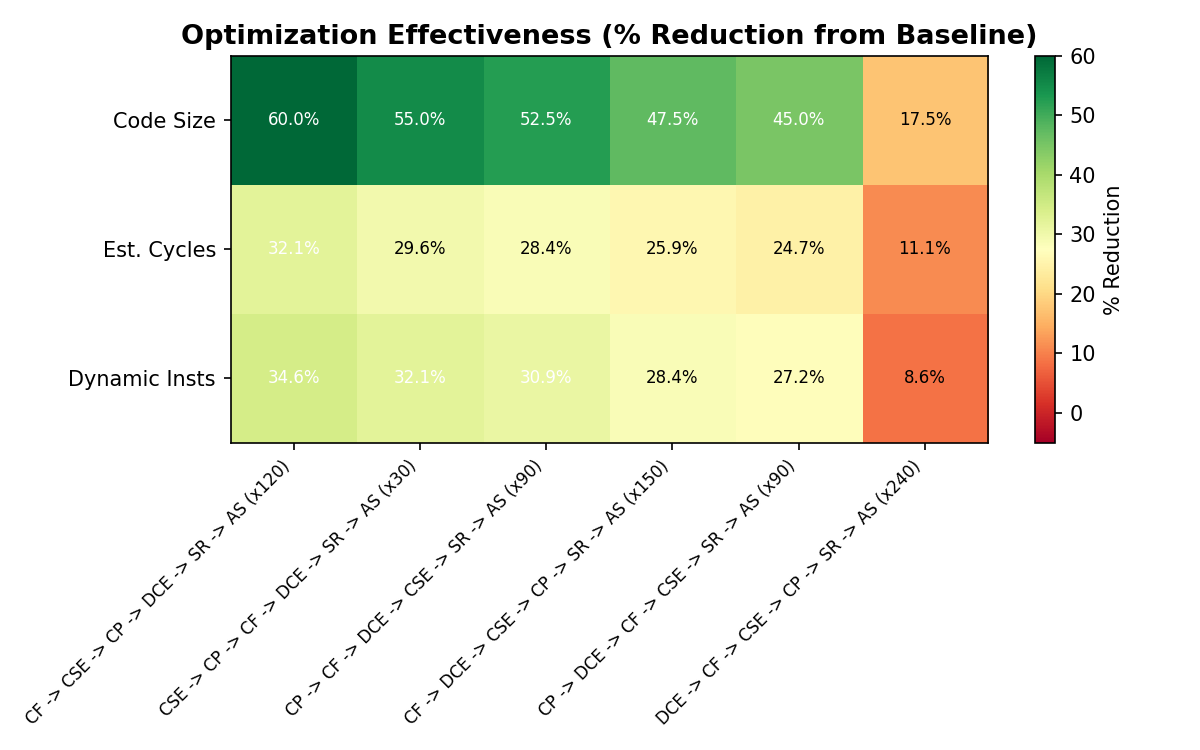
\includegraphics[width=\columnwidth]{fig/factorial_reduction_heatmap.png}
    \caption{Heatmap of optimization effectiveness showing percentage reduction from baseline across code size, estimated cycles, and dynamic instructions for each sequence.}
    \label{fig:reduction_heatmap}
\end{figure}

\subsection{Behavior of Individual Optimization Passes}
Each optimization technique exhibited distinct behavior depending on its position in the sequence. Constant Folding simplified expressions at compile time, which often enabled further optimizations. Dead Code Elimination removed unused instructions, improving code clarity and efficiency. Common Subexpression Elimination reduced redundant computations, but its effectiveness depended on prior transformations. These observations highlight the interdependency between optimization passes.

\begin{table}[!htbp]
\centering
\caption{Interaction Impact Between Optimization Passes}
\label{tab:pass_interaction}
\renewcommand{\arraystretch}{1.2}
{\small
\begin{tabularx}{\columnwidth}{@{}Xccccc@{}}
\toprule
\textbf{First Pass} & \textbf{AS} & \textbf{CF} & \textbf{CP} & \textbf{CSE} & \textbf{DCE} \\
\midrule
AS  & 0     & $+$3  & $+$2  & 0     & $-$5  \\
CF  & $-$3  & 0     & $-$1  & $-$3  & $-$11 \\
CP  & $-$2  & $+$1  & 0     & $-$2  & $-$10 \\
CSE & 0     & $+$3  & $+$2  & 0     & $-$5  \\
DCE & $+$5  & $+$11 & $+$10 & $+$5  & 0     \\
SR  & 0     & $+$3  & $+$2  & 0     & $-$5  \\
\bottomrule
\end{tabularx}
}
\end{table}

The pass interaction heatmap in Fig.~\ref{fig:pass_interaction} provides a visual representation of the pairwise interaction effects. Negative values (blue) indicate that applying pass A before B reduces code size compared to the reverse order, while positive values (red) indicate the opposite. The strongly negative values in the CF and CP rows when paired with DCE confirm that constant folding and copy propagation are most effective when applied before dead code elimination.

\begin{figure}[htbp]
    \centering
    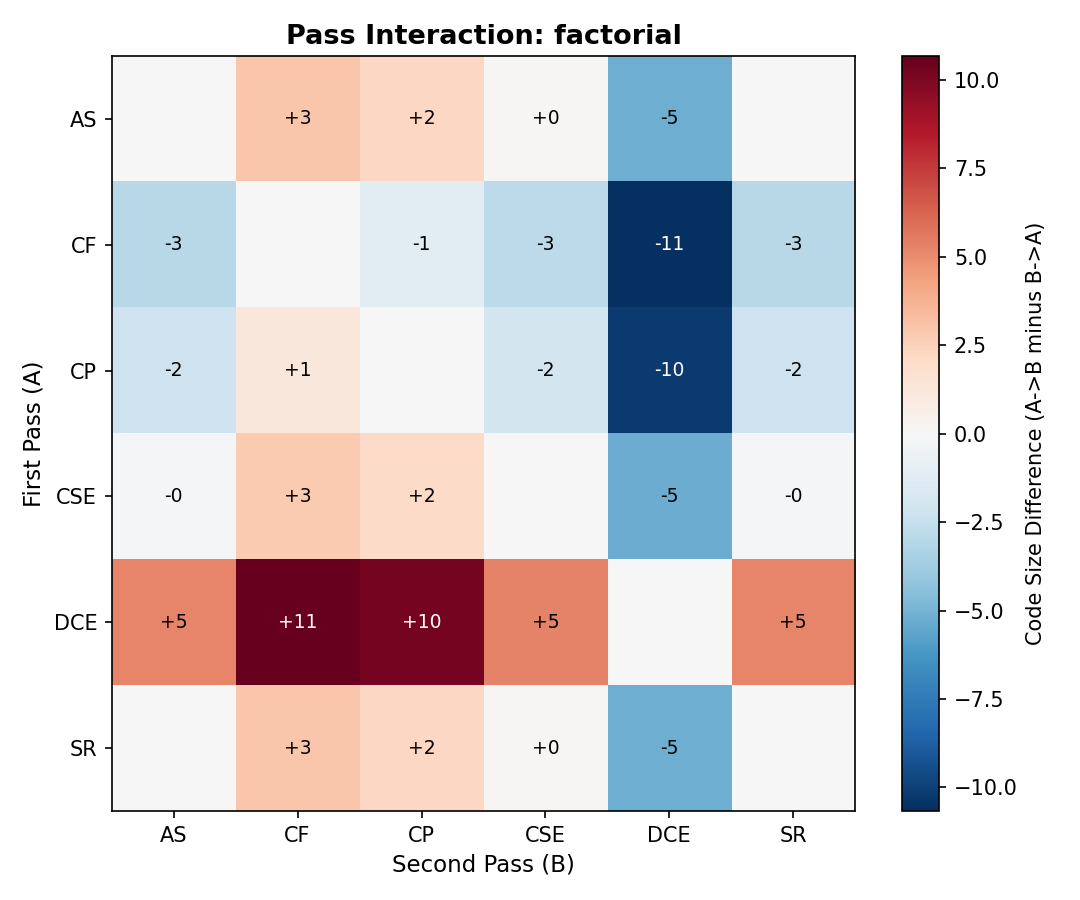
\includegraphics[width=\columnwidth]{fig/factorial_pass_interaction.png}
    \caption{Pass interaction heatmap showing the code size difference when applying pass A before pass B versus the reverse order.}
    \label{fig:pass_interaction}
\end{figure}

\subsection{Validation Using Micro-Benchmarks}
Micro-benchmark programs were used to evaluate optimization sequences under consistent conditions. The results confirmed that benchmark-driven evaluation provides a reliable way to measure optimization effectiveness. Metrics such as instruction count and estimated execution cycles allowed quantitative comparison of different phase orderings.

\begin{table}[!htbp]
\centering
\caption{Normalized Performance Metrics Relative to Baseline}
\label{tab:normalized_performance}
\renewcommand{\arraystretch}{1.2}
\begin{tabularx}{\columnwidth}{@{}Xcc@{}}
\toprule
\textbf{Sequence} & \textbf{Norm. Code Size} & \textbf{Norm. Cycles} \\
\midrule
Seq 1 & 0.40 & 0.68 \\
Seq 2 & 0.45 & 0.70 \\
Seq 3 & 0.48 & 0.72 \\
Seq 4 & 0.52 & 0.74 \\
Seq 5 & 0.55 & 0.75 \\
Seq 6 & 0.83 & 0.89 \\
\bottomrule
\end{tabularx}
\end{table}

Fig.~\ref{fig:normalized_bars} visualizes the normalized metrics, making it straightforward to compare the relative effectiveness of each sequence. The dashed baseline at 1.0 represents unoptimized code, and bars further below the baseline indicate greater optimization effectiveness. The consistent ordering across both metrics confirms the reliability of the evaluation approach.

\begin{figure}[htbp]
    \centering
    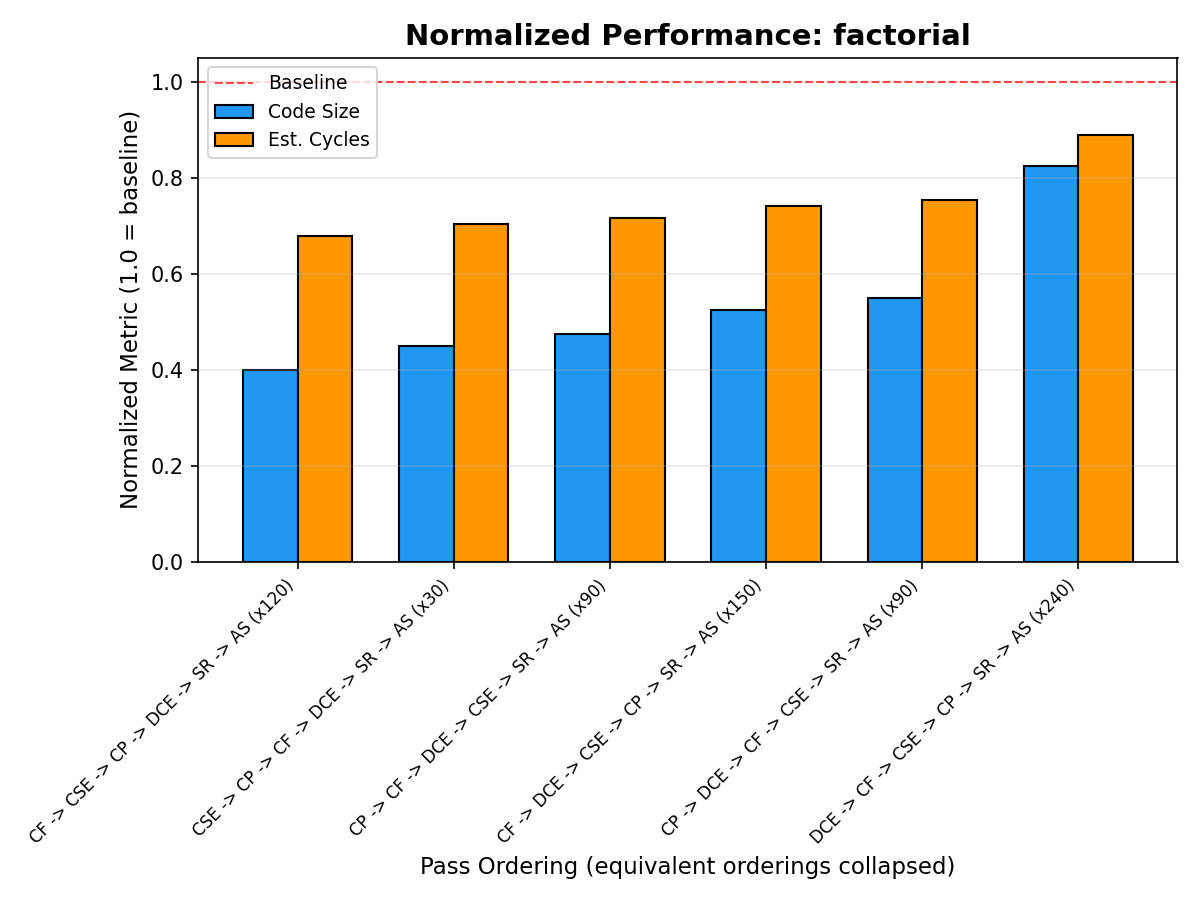
\includegraphics[width=\columnwidth]{fig/factorial_normalized_bars.png}
    \caption{Normalized performance metrics relative to the unoptimized baseline (1.0) for each optimization sequence.}
    \label{fig:normalized_bars}
\end{figure}

\subsection{System Effectiveness and Flexibility}
The custom compiler framework proved to be effective for controlled experimentation. The modular design, along with the configurable pass manager, allowed flexible reordering and selective execution of optimization passes. This made it possible to systematically analyze phase ordering behavior without the complexity of large industrial compilers.



% --- SECTION VIII: CONCLUSION ---
\section{Conclusion}
This project addressed the Phase Ordering Problem in compiler design by developing a custom, modular compiler framework that enables controlled experimentation with optimization sequences. The compiler was designed with a handwritten lexical analyzer, a recursive-descent parser, and a Three-Address Code (3AC) intermediate representation, providing a clear and structured environment for applying and analyzing optimizations.

Three fundamental optimization techniques—Constant Folding (CF), Dead Code Elimination (DCE), and Common Subexpression Elimination (CSE)—were implemented as independent and reorderable passes using a configurable pass manager. This design allowed systematic evaluation of different optimization sequences and their impact on program performance and code size.

The experimental results demonstrated that the order of applying optimization passes significantly influences the effectiveness of the compiler. Different phase sequences produced varying outcomes in terms of instruction count and estimated execution performance, highlighting the interdependency between optimization techniques. The study also revealed that no single optimization sequence is universally optimal, and the effectiveness of a sequence depends on the structure and characteristics of the input program.

Overall, the project demonstrates the importance of modular compiler design and controlled experimentation in studying complex optimization problems. The developed framework can serve as a foundation for further research, including the addition of advanced optimization techniques, automated phase ordering strategies, or integration with machine learning approaches to enhance compiler performance.

% --- SECTION IX: FUTURE WORK ---
\section{Future Work}
Possible extensions include:
\begin{itemize}
    \item Expand benchmark corpus and include real-world workloads.
    \item Integrate additional passes and study higher-order interactions.
    \item Explore ML-guided phase ordering (supervised / reinforcement approaches).
    \item Investigate runtime feedback loops and dynamic phase adaptation.
    \item Optimize interpreter and integrate low-level measurement using hardware counters for precise latency data.
\end{itemize}

% --- REFERENCES ---
\begin{thebibliography}{30}

\bibitem{ref27}
A. H. Ashouri, S. S. G. Bagi, K. Satheeskumar, T. Srikanth, J. Zhao, I. Saidoun, Z. Wang, B. Chan, and T. S. Czajkowski, 
``Protean compiler: An agile framework to drive fine-grain phase ordering,'' 
arXiv preprint, 2026.
\url{https://doi.org/10.48550/arXiv.2602.06142}

\bibitem{ref7}
J. Zhao \textit{et al.}, 
``Leveraging compilation statistics for compiler phase ordering,'' 
in \textit{Proceedings of the IEEE International Parallel and Distributed Processing Symposium (IPDPS)}, 2025.
\url{https://doi.org/10.1109/IPDPS64566.2025.00054}

\bibitem{ref25}
Y. Chen, H. Chen, Y. Yao, P. Yu, F. Xu, and X. Ma, 
``Exploiting booster pass chain for compiler phase ordering,'' 
\textit{ACM Transactions on Embedded Computing Systems (TECS)}, 2025.
\url{https://doi.org/10.1145/3755881.3755899}

\bibitem{ref30}
R. Koitz-Hristov, F. Mandl, and F. Wotawa, 
``VisOpt: Visualization of compiler optimizations for computer science education,'' 
in \textit{Proceedings of the ACM Conference}, 2025.
\url{https://doi.org/10.1145/3641554.3701832}

\bibitem{ref1}
J. Liu \textit{et al.}, 
``Efficient compiler optimization by modeling passes dependence,'' 
\textit{CCF Transactions on High Performance Computing}, 2024.
\url{https://doi.org/10.1007/s42514-024-00197-9}

\bibitem{ref2}
R. Han and H. Kim, 
``Exponentially expanding the phase-ordering search space via dormant information,'' 
in \textit{Proceedings of the ACM SIGPLAN Conference on Compiler Construction (CC)}, 2024.
\url{https://doi.org/10.1145/3640537.3641582}

\bibitem{ref3}
Y. Wang, H. Chen, and K. Wang, 
``Beyond the phase ordering problem: Finding the globally optimal code with respect to optimization phases,'' 
arXiv preprint, 2024.
\url{https://doi.org/10.48550/arXiv.2410.03120}

\bibitem{ref4}
F. Huemer, D. Leopoldseder, A. Prokopec, R. Mosaner, and H. Mössenböck, 
``Taking a Closer Look: An Outlier-Driven Approach to Compilation-Time Optimization,'' 
in \textit{Proceedings of the 38th European Conference on Object-Oriented Programming (ECOOP)}, 2024.
\url{https://doi.org/10.4230/LIPIcs.ECOOP.2024.20}

\bibitem{ref5}
H. Ahmed, M. F. Hyder, M. F. ul Haque, and P. C. Santos, 
``Exploring compiler optimization space for control flow obfuscation,'' 
\textit{Computers \& Security}, 2024.
\url{https://doi.org/10.1016/j.cose.2024.103704}

\bibitem{ref6}
A. Schmitz \textit{et al.}, 
``Parallel pattern compiler for automatic global optimizations,'' 
\textit{Parallel Computing}, 2024.
\url{https://doi.org/10.1016/j.parco.2024.103112}

\bibitem{ref14}
F. Fernandes dos Santos, L. Carro, F. Vella, and P. Rech,
"Assessing the Impact of Compiler Optimizations on GPUs Reliability,"
\textit{ACM Transactions on Architecture and Code Optimization (TACO)},
vol. 21, no. 2, 2024.
\url{https://doi.org/10.1145/3638249}

\bibitem{ref13}
H. Zhou \textit{et al.}, 
``Semantic ontology enabled modeling, retrieval and inference for incomplete mobile trajectory data,'' 
\textit{Future Generation Computer Systems}, 2023.
\url{https://doi.org/10.1016/j.future.2023.03.012}

\bibitem{ref22}
M. Zhu and D. Hao, 
``Compiler auto-tuning via critical flag selection,'' 
in \textit{Proceedings of the IEEE/ACM International Conference on Automated Software Engineering (ASE)}, 2023.
\url{https://doi.org/10.1109/ASE56229.2023.00209}

\bibitem{ref24}
A. Pe\v{c}im\'{u}th, D. Leopoldseder, and P. T\u{u}ma, 
``Diagnosing compiler performance by comparing optimization decisions,'' 
in \textit{Proceedings of the ACM SIGPLAN Conference}, 2023.
\url{https://doi.org/10.1145/3617651.3622994}

\bibitem{ref26}
R. Han and H. Kim, 
``Exponentially expanding the compiler phase-ordering problem's search space through the learning of dormant information,'' 
2023.
\url{https://openreview.net/pdf?id=frjDLUebFY}

\bibitem{ref29}
C. Shewale, S. B. Shinde, Y. B. Gurav, R. J. Patil, and S. U. Kadam, 
``Compiler optimization prediction with new self-improved optimization model,'' 
\textit{International Journal of Advanced Computer Science and Applications (IJACSA)}, vol. 14, no. 2, 2023.
\url{https://doi.org/10.14569/IJACSA.2023.0140267}

\bibitem{ref8}
S. Jain \textit{et al.}, 
``POSET-RL: Phase ordering for optimizing size and execution time using reinforcement learning,'' 
in \textit{Proceedings of the IEEE ISPASS}, 2022.
\url{https://doi.org/10.1109/ISPASS55109.2022.00012}

\bibitem{ref10}
L. Chen \textit{et al.}, 
``Automated test-based learning and verification of performance models for microservices systems,'' 
\textit{Journal of Systems and Software}, 2022.
\url{https://doi.org/10.1016/j.jss.2022.111225}

\bibitem{ref11}
X. Liu and Y. Zhang, 
``A large-scale parallel fluid-structure interaction computing platform for simulating structural responses to a detonation shock,'' 
\textit{Software: Practice and Experience}, 2022.
\url{https://doi.org/10.1002/spe.3051}

\bibitem{ref28}
H. Liu, J. Xu, S. Chen, and T. Guo, 
``Compiler optimization parameter selection method based on ensemble learning,'' 
\textit{Electronics}, vol. 11, no. 15, 2022.
\url{https://doi.org/10.3390/electronics11152452}

\bibitem{ref23}
S. Kloibhofer, 
``Run-time data analysis to drive compiler optimizations,'' 
\textit{ACM Transactions on Architecture and Code Optimization (TACO)}, 2021.
\url{https://doi.org/10.1145/3484271.3484974}

\bibitem{ref9}
S. VenkataKeerthy \textit{et al.}, 
``IR2Vec: LLVM IR based scalable program embeddings,'' 
\textit{ACM Transactions on Architecture and Code Optimization (TACO)}, 2020.
\url{https://doi.org/10.1145/3418463}

\bibitem{ref12}
Q. Huang \textit{et al.}, 
``AutoPhase: Compiler phase-ordering for high-level synthesis,'' 
arXiv preprint, 2020.
\url{https://doi.org/10.48550/arXiv.2003.00671}

\bibitem{ref15}
A. H. Ashouri \textit{et al.}, 
``MiCOMP: Mitigating the compiler phase-ordering problem using optimization subsequences and machine learning,'' 
\textit{ACM Transactions on Architecture and Code Optimization (TACO)}, 2017.
\url{https://doi.org/10.1145/3131284}

\bibitem{ref17}
A. Singh and P. Sharma, 
``Predictive modeling methodology for compiler phase-ordering,'' 2016.
\url{https://doi.org/10.1145/2872421.2872424}

\bibitem{ref20}
R. Nobre, L. G. A. Martins, and J. M. P. Cardoso, 
``A graph-based iterative compiler pass selection and phase ordering approach,'' 
in \textit{Proceedings of the IEEE International Parallel and Distributed Processing Symposium (IPDPS)}, 2016.
\url{https://doi.org/10.1145/2907950.2907959}

\bibitem{ref16}
C. Lattner and V. Adve, 
``LLVM: A compilation framework for lifelong program analysis and transformation,'' 
in \textit{Proceedings of the International Symposium on Code Generation and Optimization (CGO)}, 2004.
\url{https://doi.org/10.1109/CGO.2004.1281665}

\bibitem{ref19}
P. Kulkarni \textit{et al.}, 
``Fast searches for effective optimization phase sequences,'' 
in \textit{ACM SIGPLAN Notices}, 2004.
\url{https://doi.org/10.1145/996893.996863}

\bibitem{ref18}
K. D. Cooper, T. J. Harvey, and L. Torczon, 
``Compiler-based code-improvement techniques,'' 
in \textit{Handbook of Computer Science and Engineering}, 2002.
\url{https://www.cs.tufts.edu/~nr/cs257/archive/keith-cooper/survey.pdf}

\bibitem{ref21}
D. F. Bacon, S. L. Graham, and O. J. Sharp,
"Compiler transformations for high-performance computing," \textit{ACM Computing Surveys}, 1994.
\url{https://doi.org/10.1145/197405.197406}

\end{thebibliography}

\end{document}
